O menino Araújo, filho de biólogos, sempre foi fascinado por espécies cobras grandes que eram criadas no cativeiro da casa. Hoje pela manhã ele ganhou um dominó no bingo da escola e, já em casa, formulou o jogo ``A Maior Cobra Legal de Dominós''. A regra desta atividade é bem simples, formar a maior cobra de dominós usando a regra de encaixe das peças. Por exemplo, se ele usa todas as peças com até 4 valores, uma possível maior cobra de se formar teria 9 peças com a seguinte configuração:

\begin{center}
  | 0-0 | 0-1 | 1-1 | 1-2 | 2-2 | 2-0 | 0-3 | 3-3 | 3-1 |
\end{center}

Observe que a peça 2-3 (ou 3-2, a peça é a mesma) não foi possível de ser usada.

Agora, se ele usa todas as peças com até 5 valores, uma possível maior cobra de se formar teria 15 peças com a seguinte configuração:

\begin{center}
  | 0-0 | 0-1 | 1-1 | 1-2 | 2-2 | 2-0 | 0-3 | 3-3 | 3-1 | 1-4 | 4-4 | 4-2 | 2-3 | 3-4 | 4-0 |
\end{center}

Curioso que é, o menino Araújo solicitou a ajuda dos programadores da Maratona Mineira para criar um programa com a seguinte missão: Dado o valor máximo de unidades de um jogo de dominó, informe qual é o tamanho da maior cobra legal de dominós.

\begin{center}
  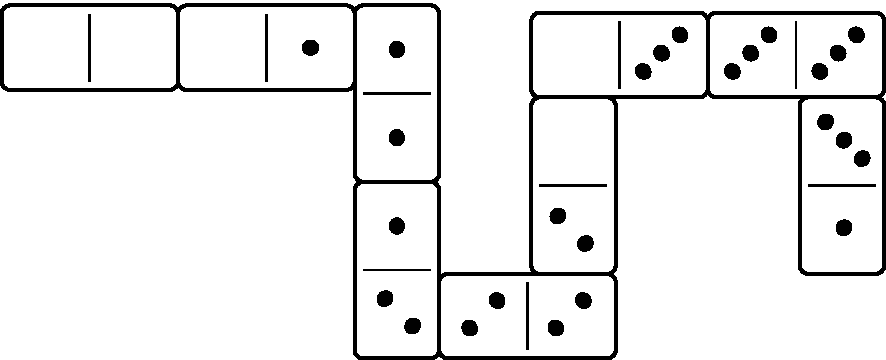
\includegraphics[width=0.7\linewidth]{\CWD/dominos.pdf}
\end{center}


\section*{Entrada}

Há vários casos de teste. Cada caso de teste possui uma linha com um número inteiro $N$ que representa o número de unidades máxima que o jogo de dominó possui. Os casos de teste encerram quando for informado o valor $0$ para $N$.

\section*{Saída}

Para cada caso de teste, deve ser impresso uma linha no formato "Caso $I$: $T$", em que $I$ representa o índice do caso e $T$ o tamanho máximo legal que a cobra pode assumir.

\section*{Restrições}

$$1 \leq N \leq 5000$$

\section*{Exemplos}

Entrada

1
4
5
7
10
0

Saída

Caso 1: 1
Caso 2: 9
Caso 3: 15
Caso 4: 28
Caso 5: 51

\exemplo
